\documentclass[12pt, hyperref={bookmarks=false}, show notes]{beamer}
% Text
        \usepackage[T1]{fontenc}
        \usepackage[utf8]{inputenc}
        \usepackage[english]{babel}
        \usepackage[bitstream-charter]{mathdesign} % Serif font (Charter BT).
        \usepackage[scaled=0.84]{DejaVuSansMono} % Monospaced font.
        \def\sfdefault{SourceSansPro-TLF} % Sans serif font.
        \usepackage{textcomp}

% Maths
  \usepackage{amsmath}
  \usepackage{mathtools}
  \usepackage{siunitx}
  % Vector command
  \newcommand{\omatrix}[1]{\ensuremath{\boldsymbol{#1}}}

% Graphics
  \usepackage{graphicx}
  \usepackage[caption=false]{subfig}
        \usepackage{tikz}
  \usepackage{pgfplots}
  \pgfplotsset{compat=1.10}
        % ADD TIKZ LIBRARIES
  \usetikzlibrary{calc}
  \usetikzlibrary{arrows.meta}
  \usepackage{tikz-qtree}
  \usetikzlibrary{decorations.pathmorphing}
  \usetikzlibrary{matrix,shapes,positioning,fit}
  \usepgfplotslibrary{external}
  \tikzexternalize[prefix=graphics/tikz/]
  \tikzexternaldisable % Disable by default
  \usepackage{tabularx}
  \usepackage{pgfgantt}

        \usepackage{xcolor}
    \definecolor{color1}{cmyk}{100,50,0,0}   % blue
    \definecolor{color2}{cmyk}{0,80,100,0}   % vermillion
    \definecolor{color3}{cmyk}{97,0,75,0}    % blueish green
    \definecolor{color4}{RGB}{204,121,167}    % reddish purple
    \definecolor{color5}{RGB}{230,159,0}   % orange
   \usepackage{colortbl}
% Misc
\usepackage{booktabs}
\usepackage{enumerate}
\usepackage{pdfpages}
\usepackage{pgfpages}
\usepackage{setspace}
%\usepackage{multimedia}

\setbeamertemplate{navigation symbols}{}
\setbeamertemplate{caption}{\raggedright\insertcaption\par}
%\setbeamertemplate{bibliography item}[text]

%\usepackage{caption}
\usetheme{/amsterdam}
\date{October 11, 2016}

\usepackage{beamertheme/handoutWithNotes}
% Uncomment for handouts. Add \documentclass[12pt,handout]{beamer}
%\pgfpagesuselayout{4 on 1 with notes}[a4paper,border shrink=5mm]
% Comment for handouts.
\setbeameroption{show notes on second screen=right}

% Table of content dybde (0-index)
%\setcounter{tocdepth}{1}

% BibLaTeX
%\usepackage{csquotes}
%\usepackage[
%backend=bibtex,
%citestyle=numeric,
%bibstyle=numeric,
%maxcitenames=3,
%maxbibnames=99,
%url=true]{biblatex}
%\addbibresource{../rapport/references/refs.bib}
%\addbibresource{extrasources.bib}
%\usepackage{../style/biblatex_custom_formatting}

\graphicspath{{graphics/}{../../Report/graphics/}}

\begin{document}

%\captionsetup[figure]{font=small,singlelinecheck=off,justification=raggedright}

\title[Sequence to Sequence Learning
with Neural Networks]{TrashVision}
\author[\insertframenumber /\inserttotalframenumber]{SW703E15}

\begin{frame}
\Huge Sequence to Sequence Learning
with Neural Networks\\
\small by Ilya Sutskever, Oriol Vinyals, and Quoc V. Le\\
\end{frame}

% PUT INPUTS HERE
\begin{frame}
	\frametitle{Motivation}
	\begin{itemize}
		\item The Problem
		\begin{itemize}
			\item Deep Neural Networks
			\begin{itemize}
				\item Requires fixed dimensionality on input and output
			\end{itemize}
		\end{itemize}
		\item The Solution
		\begin{itemize}
			\item Recurrent Neural Network
			\begin{itemize}
				\item Can take a sequence of inputs
				\item Can map a sequence to a fixed size vector
			\end{itemize}
		\end{itemize}
	\end{itemize}


	\note{
		\begin{itemize}
			\item Requires fixed dimensionality on input and output
		\end{itemize}
	}
\end{frame}

\begin{frame}
	\frametitle{The solution}
	\begin{itemize}
		\item Recurrent Neural Network
		\begin{itemize}
			\item Directed cycle
			\item Can take a sequence of inputs
			\item Can map a sequence to a fixed size vector
		\end{itemize}
	\end{itemize}
	\note{
		\begin{itemize}
			\item Holds a cycle
			\item Can take a sequence of inputs
		\end{itemize}
	}
\end{frame}

\begin{frame}
	\frametitle{Recurrent Neural Network}
	\begin{figure}
		\centering
		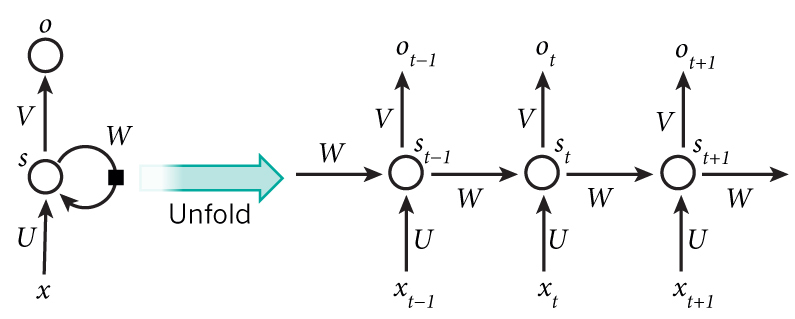
\includegraphics[scale=0.3]{rnn.jpg}
	\end{figure}
\end{frame}

\begin{frame}
	\frametitle{Long short term memory network}
	\begin{figure}
		\centering
		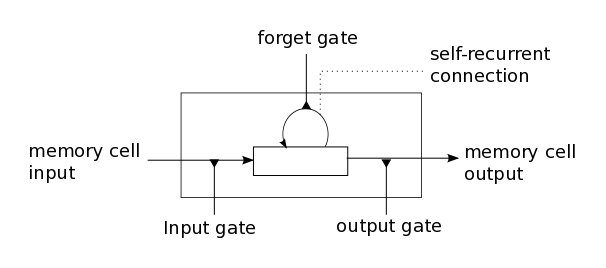
\includegraphics[scale=0.5]{lstm_memorycell.png}
	\end{figure}
\end{frame}

\begin{frame}
	\frametitle{Results}
	\begin{figure}
		\centering
		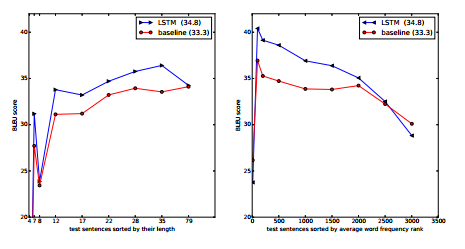
\includegraphics[scale=0.8]{results.png}
	\end{figure}
\end{frame}

\section*{}

\end{document}
